\section{Discussion} 
\label{sec:discussion}

\subsection{What's best on a $>1$ year horizon for planet detections?}
\label{sec:gtr_1yr_horizon}

% Contextualize importance of thinking beyond just 1 yr Extended Mission
\tesss orbit is stable, in principle, for more than 1000 years~\citep{gangestad_high_2013}.
While minor mechanical failures should be expected on the timescale of a few years, it is plausible that the spacecraft could outlive both the 2-year Primary Mission and the 1-year Extended Mission.
Therefore, when choosing any particular plan for a 1-year Extended Mission, it makes
sense to also consider the implications of an even longer Extended Mission.

% Preliminary discussion of immediate extensibility
A simple point is that \nhemi, \npole, and \shemiAvoid\:can all be inverted to their southern or northern complements for a fourth year of observing.
This will yield a comparable number of new planets to what they find in year 3 ($\mathcal{O}(1300)$ with $R_p<4R_\oplus$).
This argues strongly to continue observing the entire sky, rather than focusing on a single ecliptic hemisphere after the Primary Mission's completion.
This would continue \tesss role as a planet-discovery machine, while also addressing the practical matter of refining ephemerides in order to enable detailed characterization with suitable instruments.
%Leave the detailed characterization for \jwst, Spitzer, HST, ground-based ELTs, and posterity.

The \elong, \eshort, and \hemis\:scenarios are less obviously extensible to multiple years.
The main reasons to return to the ecliptic after performing \elong\:or \eshort\:would be to make \tesss survey truly `all-sky', and to complete all possible \ktwo follow-up observations (see discussion below).
Of course, this would need to happen during intervals in which the Moon and Earth were not in the way.
%Continuous observations have serious value. 

% Move on to very-long term comments.
Any of our proposed scenarios could simply be repeated indefinitely,
as could possible two-year Extended Missions in which our scenarios 
would be followed by their respective complement hemispheres.
Slightly different trade-offs may arise when comparing two-year
Extended Missions.
For instance, consider: (1) two years of \hemis; (2) repeating the 
Primary Mission for two years.
If we repeat the Primary Mission over 2 years, the northern
and southern CVZs each get 1 year of continuous observation.  If we
execute \hemis\:for 2 years, the northern and southern `long viewing
zones' each get 2 years of 14-day windowed observations.  The latter
case allows 2-transit detections of $P\lesssim1$ year planets over
$2\%$ of the sky.  The former allows 2-transit detections of
$P\lesssim6$ month planets over $1\%$ of the sky.  This simple
consideration of course misses that point that data obtained from
repeating the Primary Mission would be less subject to aliasing
problems and would have fewer period ambiguities.  However
repeating \hemis\:for two years might be a middle ground between the
two extreme strategies ``repeat \npole\:indefinitely'' and ``repeat
the Primary Mission indefinitely''.

A longer-term question is ``when will \tess hit the point of
diminishing returns?''  The `low-hanging fruit' of small planets
transiting bright stars at short orbital periods will eventually be
found if \tess continues to observe the same sky.  The most important
qualitative point of this memo, made in Fig.~\ref{fig:snrf_histogram},
is that after \tesss Primary Mission there will be many objects
remaining for which merely doubling the number of observed transits
will enable their detection.  Eventually though, the peak of the
phase-folded SNR distribution shown in Fig.~\ref{fig:snrf_histogram}
will shift past the detection threshold, and more observations will
only allow us to probe out to longer orbital periods and dimmer stars.
No detailed study has yet quantified when \tess will reach this
operating regime.

\subsection{The ephemeris problem}
\label{sec:ephemeris_times}

\paragraph{Analytic motivation}

For follow-up observations, we will often need to predict future times
of transits or occultations, ideally with an accuracy of an hour or
less. After enough time has passed that the uncertainty has grown to a
significant fraction of the orbital period, we say that the ephemeris
has gone ``stale'', presenting a major obstacle to many follow-up
programs. For \tesss ground-based follow-up campaign, the problem of a
stale ephemeris could double or triple the amount of observing time
that is required for a successful result.  Likewise, for planning
space-based observations, for which observing time is always scarce,
it is extremely important to have a reliable and accurate ephemeris.
For mass determination through the Doppler method, a stale transit
ephemeris adds uncertainty to the planetary mass measurements, by
increasing the number of effectively free parameters.

Consider then the problem of estimating $\sigma_{t_c}(T_x)$, the
uncertainty of the mid-transit time $\sigma_{t_c}$ for a given planet
at some time $T_x$ following its last-observed transit.  We begin
analytically: assume that the planet has $N_\mathrm{tra}=2$ observed
transits, spaced an orbital period $P=14$ days apart. Because that
period is one half the nominal \tess dwell time of a given pointing,
it represents the shortest period for which typically
$N_\mathrm{tra}=2$, and as such is the worst-case scenario for predicting
the times of future transits, amongst cases with $N_\mathrm{tra}>1$.
Given two mid-transit times, each measured with the time's uncertainty
$\sigma_0$, separated by $P$, the uncertainty of a future mid-transit
time can be derived by standard least-squares fitting and propagation
of errors (\textit{e.g.}~\citet{lyons_practical_1991}, Equation 2.18):

\begin{equation}
	\sigma_{t_c}(T_x) = \sigma_0 \sqrt{1 + 2 T_x / P + 2 (T_x / P)^2 }
\end{equation}
Note that for observing future transits, $E \equiv T_x / P$ is an integer, and the above equation can be re-expressed:
\begin{equation}
	\sigma_{t_c}(E) = \sigma_0 \sqrt{1 + 2 E + 2 E^2 },
\end{equation}
which is bounded by the simpler approximation: 
\begin{equation}
	\sigma_{t_c}(E) \lesssim \sigma_0 \left(1+\sqrt{2} E\right), 
\end{equation}
which is exact at $E=0$, has a maximum 8\% fractional error at $E=1$, and becomes increasingly accurate as $E$ increases. By $E=20$, the fractional error of the latter approximation is less than 1\%.

For $T_x = 2$ years and $P = 2$ weeks, then $E \approx 50$, so $\sigma_{t_c}\approx 75\sigma_0$. 
At 2-minute cadence, a typical value for the per-transit timing uncertainty is $\sigma_0 = 4$ minutes, and the predicted uncertainty on its mid-transit time is 5 hours two years later or 10 hours four years later. This leads to a simple rule of thumb: % my oom is 5 minutes. Peter's is 2 minutes. The analytics are 5 minutes. I'll take the analytics.
\begin{quotation}
  For a two-transit super-Earth, the uncertainty in the predicted transit time, in hours, is numerically equal to about
  2$Y$, where $Y$ is the number of years after the Primary Mission.
\end{quotation}
If the transits are observed only at 30-minute cadence, then uncertainty will be roughly 4 times greater: $\sigma_0 \sim 16$ minutes. 
This claim (``$4\times$ greater'') is based on Figure 9 of~\citep{price_transit_2014}, a plot of the effects of finite cadence on timing precision. % note that they're using kepler data here 
We compared the precisions of 2-min and 30-min cadences for their specific example of $P=10$ days and a dwell time of 1 month.

On the other hand, Fig.~\ref{fig:Ntra_hist_primary} shows that 7 in 8 of the planets detected by \tesss Primary Mission will have $N_\mathrm{tra}>3$ and so their ephemerides should be better than the example derived analytically above.
Rather than generalize the analytic equations, we resort to numerical simulations in order to predict the uncertainties of mid-transit times for planets expected to be discovered by \tesss Primary Mission.

\paragraph{Numerical analysis}
We start with the analytic form~\citet{price_transit_2014} derive for the per-transit uncertainty on the mid-transit time $\sigma_0$:
$$
\sigma_{0} = \frac{1}{Q} \sqrt{ \frac{\tau T}{2} } \left( 1 - \frac{t}{3\tau} \right)^{-1/2}
$$
when $\tau\geq t$ and 
\begin{equation}
	\sigma_{0} = \frac{1}{Q} \sqrt{\frac{t T }{2}} \left( 1 - \frac{\tau}{3t} \right)^{-1/2}
	\label{eq:price_rogers}
\end{equation}
when $t > \tau$,
where $Q$ is the SNR per transit, $t$ is the cadence, $T$ is the transit duration, and $\tau$ is the ingress (or egress) time.
We have all the later terms from our yield simulation, and show the resulting distribution of $\sigma_0$ in Fig.~\ref{fig:uncertainty_tc_hist}.
Indeed, our suggested $\sigma_0$ of about 4 minutes for postage stamps and 16 minutes for full frame images is reasonable, which is good because we computed the former from the $t\rightarrow0$ limit of Eq.~\ref{eq:price_rogers} originally derived by~\citet{carter_analytic_2008}.
\begin{figure}[!t]
	\centering
	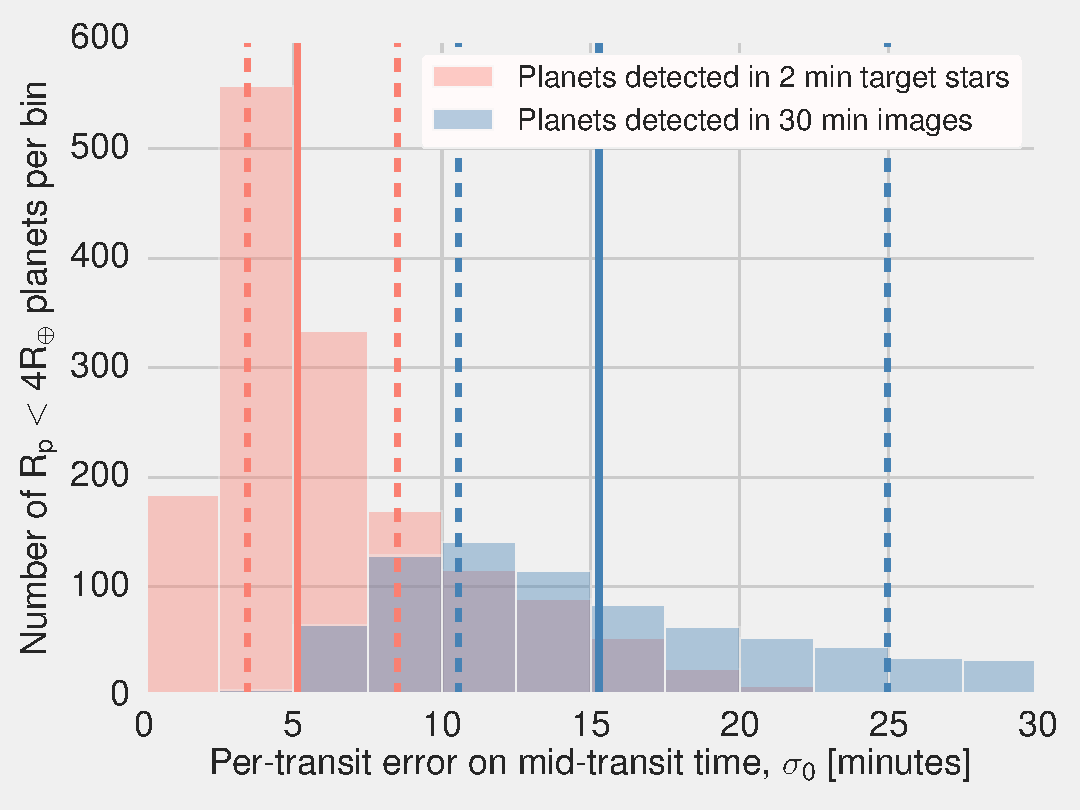
\includegraphics[scale=1.]{figures/mid_transit_time_vs_cadence.pdf}
	\caption{Uncertainty of mid-transit time on a single transit, $\sigma_{t_c}$, for all detected $R_p<4R_\oplus$ planets from the Primary Mission as computed from Eq.~\protect\ref{eq:price_rogers}.
		Solid lines are medians, dashed lines are 25$^\mathrm{th}$ and 75$^\mathrm{th}$ percentiles.
	}
	\label{fig:uncertainty_tc_hist}
\end{figure}
\begin{figure}[!t]
	\centering
	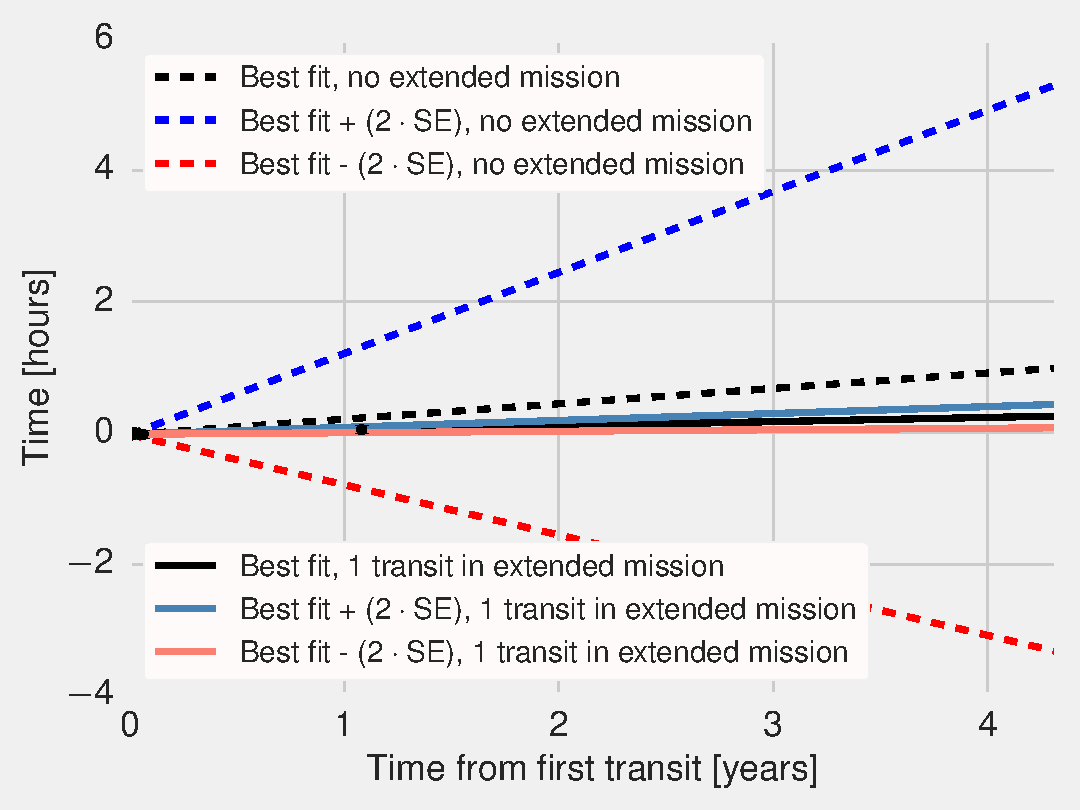
\includegraphics[scale=1.]{figures/lowering_uncertainty_on_midtransit_via_extra_point.pdf}
	\caption{	Observed mid-transit times (dots) and best fits to a linear ephemeris (lines).
		The dashed lines fit 4 data points from a nominal planet.
		The solid lines do the same, but with an additional transit observed one year
		later.
		`SE' is the standard error on the slope which multiplied by 1.96 (rounded to 2 in the legend) gives a 95\% confidence interval between the blue and orange lines.
	}
	\label{fig:lowering_uncertainty_tc}
\end{figure}

Given the distributions on per-transit uncertainty of $t_c$, we then took an example planet with 4 transits.
We drew ``observed'' mid-transit times from a Gaussian with zero mean and standard deviation $\sigma_{0}$, and then ran a linear least squares regression. 
We then added just one data point 1 year after the final observed transit, and repeated the regression.
This produces a cartoon-plot, Fig.~\ref{fig:lowering_uncertainty_tc}, which confirms two expected points:
\begin{enumerate}
	\item Years after the initial discovery, the uncertainty of mid-transit time is of order hours.
	\item If we detect an additional transit 1 year after the final observed transit from the Primary Mission, the uncertainty on the mid-transit time decreases by an order of magnitude.
\end{enumerate}

\begin{figure*}[!t]
	\centering
	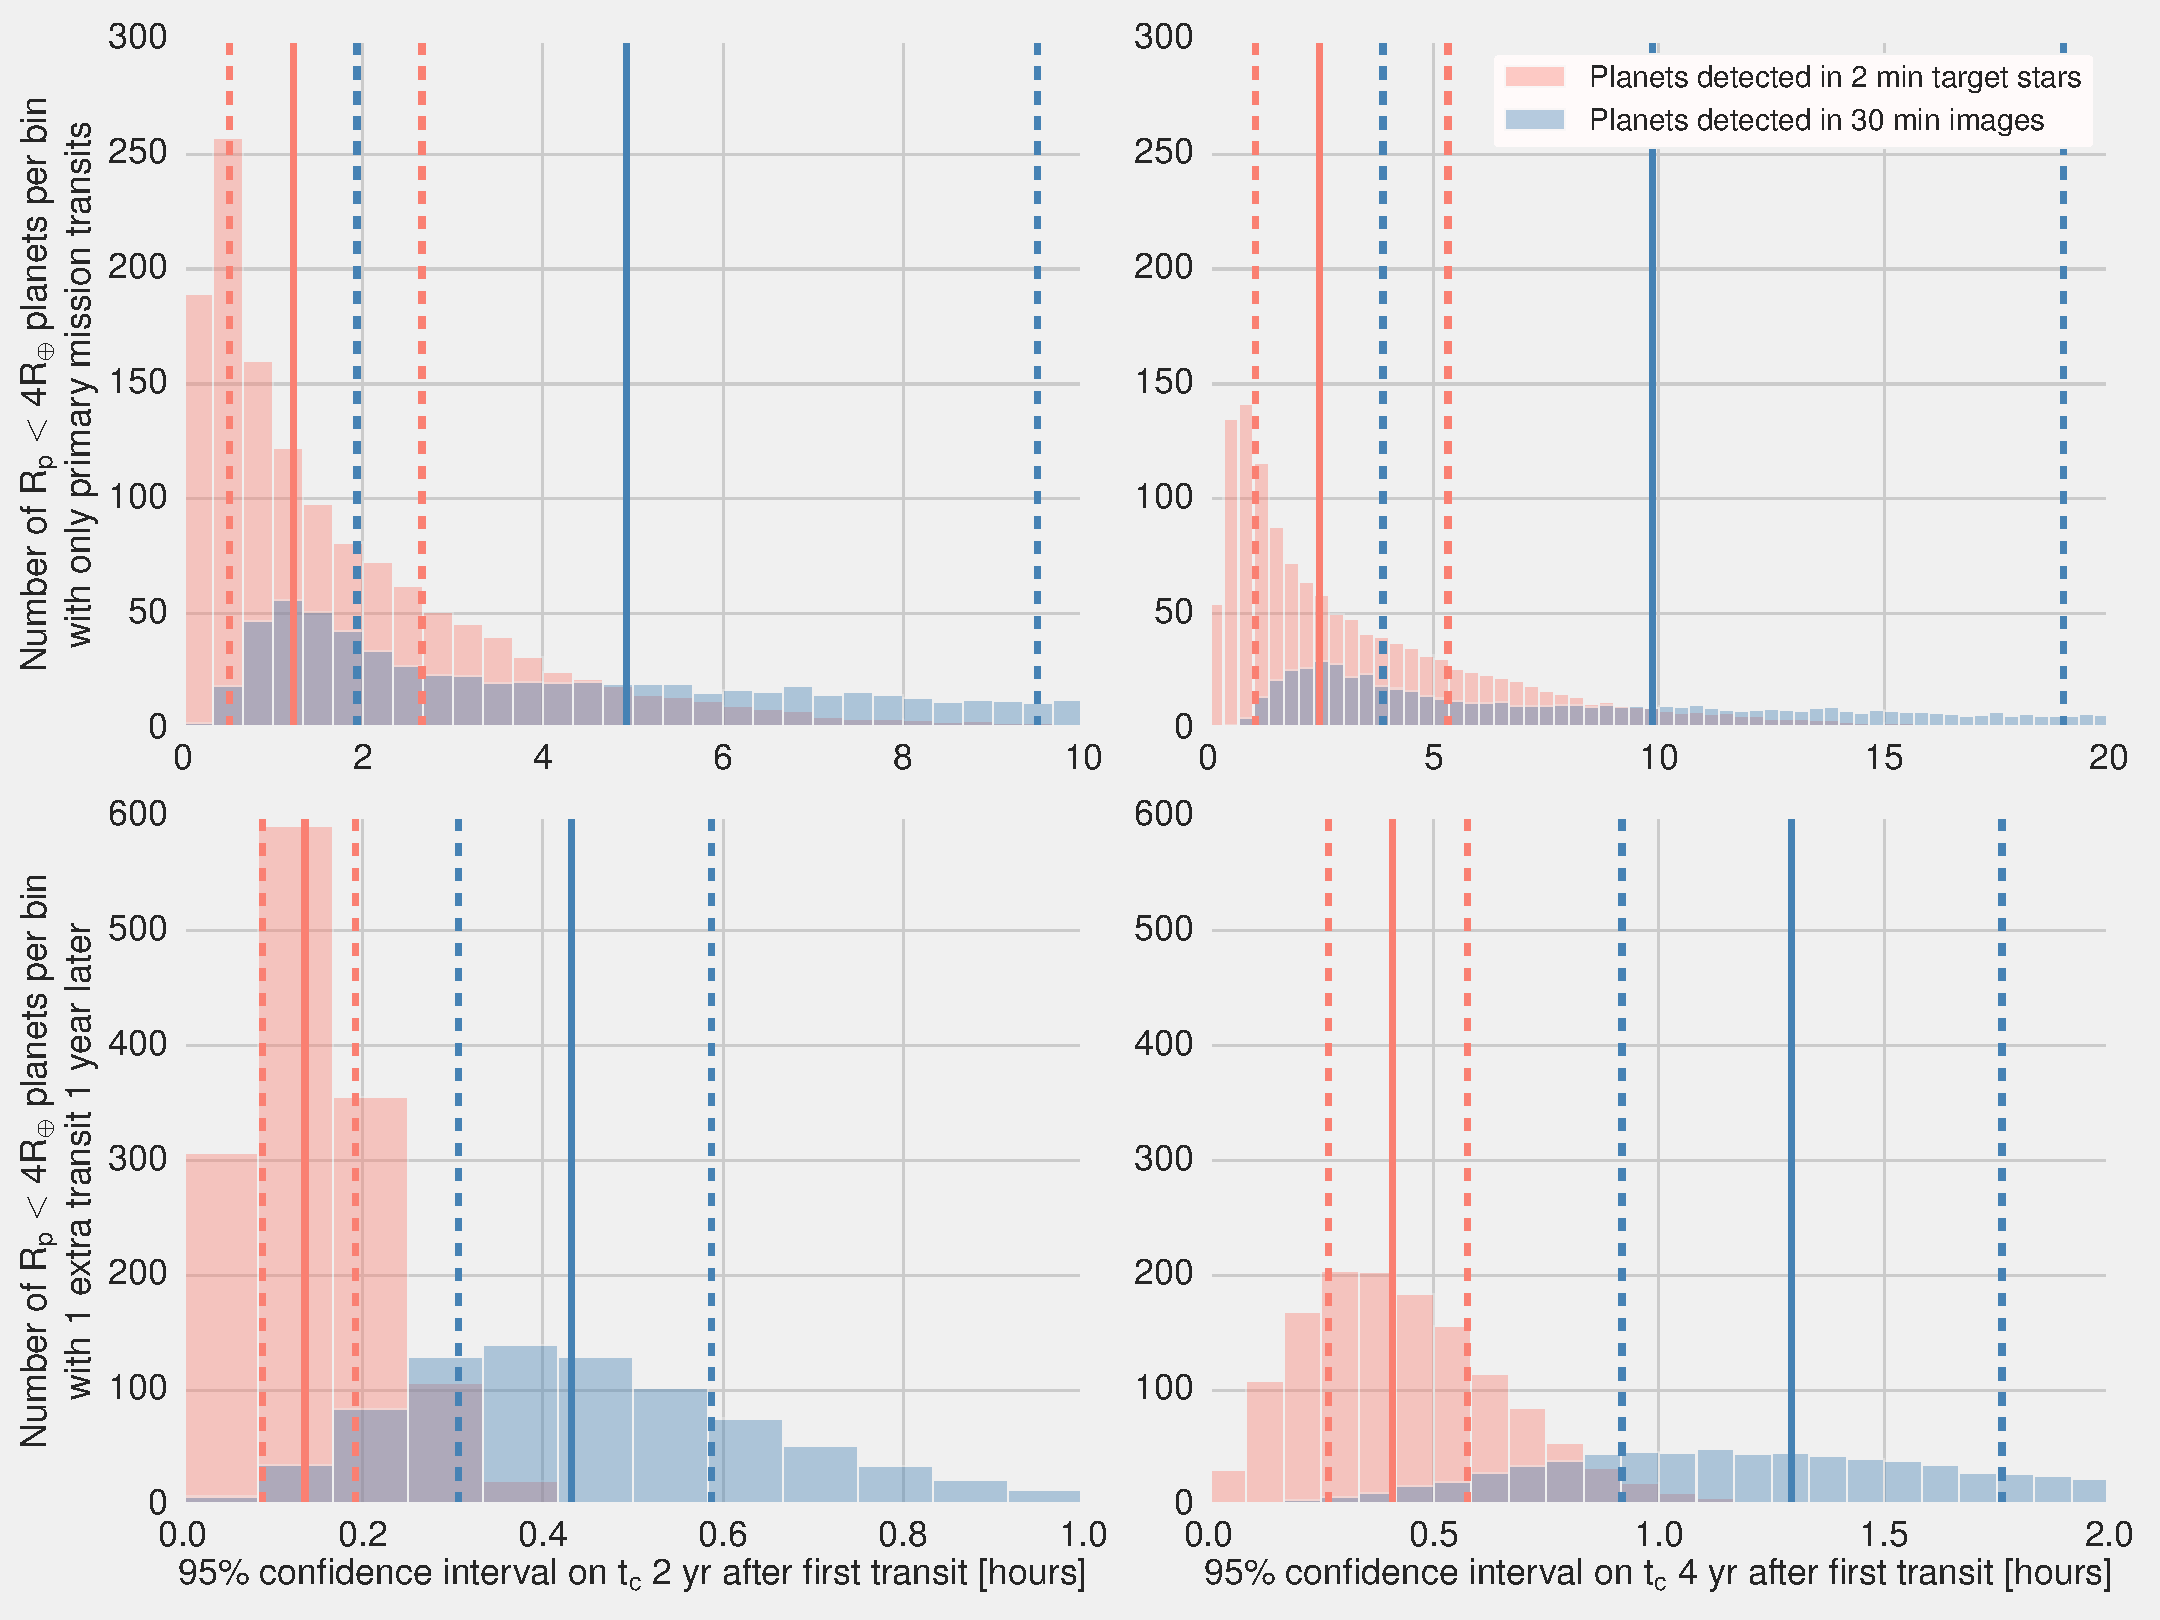
\includegraphics[scale=1.]{figures/confidence_interval_gets_better.pdf}
	\caption{\textit{Top row}: histogram of 95\% confidence intervals 2 (\textit{left}) and 4 (\textit{right}) years following the first detected transit in the Primary Mission.
		20 minute bins.
		\textit{Bottom row}: histogram of 95\% confidence intervals 2 (\textit{left}) and 4 (\textit{right}) years following the first detected transit in the Primary Mission, but with an additional data point added to the analog of Fig.~\protect\ref{fig:lowering_uncertainty_tc} one year after the transit in the initial time series (5 minute bins).
		Note that the top row's timescale is an order of magnitude greater than the bottom row.
		Solid lines are medians, dashed lines are 25$^\mathrm{th}$ and 75$^\mathrm{th}$ percentiles.
	} %all in ephemeris_uncertainties.ipynb
	\label{fig:conf_interval_gets_better}
\end{figure*}
We proceed by repeating the above procedure for every planet, and evaluate typical 95\% confidence intervals (``uncertainties'', loosely) for $t_c$, at typical times after the first transits, for all of our detected planets.
Specifically, we take them at $T_x=2$ and $4$ years, and get Fig.~\ref{fig:conf_interval_gets_better}.
This figure confirms (top left panel) our analytic expectation that the uncertainty of mid-transit times in hours should be somewhat less than twice the number of years after \tess first observes the planet at 2-min cadence, since most such planets have $N_\mathrm{tra}\geq4$.
It also confirms our rough expectation that the uncertainty on FFI mid-transit times is roughly 4 times that of postage stamps, although the uncertainties on FFIs have a much more uniform tail.

More importantly, Fig.~\ref{fig:conf_interval_gets_better} emphasizes the importance of refining \tesss ephemerides: if we do not, the typical \tess planet will have many hours of uncertainty on its mid-transit time a few years following its detection.
If we do follow-up, we will know when the planet transits to $\lesssim1$ hour for many more years.
This argues strongly for an Extended Mission which, whether over 1 or 2 years, re-observes many if not all of the targets that \tess detects in its Primary Mission. 
The smallest-radius Earths and super-Earths may otherwise be much more difficult
to follow up, due to a stale ephemeris.


\subsection{Risks and caveats}
\label{sec:risks_caveats}
\paragraph{Risk that planet detection simulation gets yield wrong:}
What is the risk that we over or under-estimated \tesss planet yield, either in the Primary Mission, or in any given Extended Mission?
We summarized the assumptions that went into our yield calculations in Sec.~\ref{sec:input_assumptions}.
We made them believing that they were all good enough for useful relative comparisons of different sky-scanning scenarios,
even if they are not correct in absolute terms to better than $\sim$50\%.
%Fortunately, we can be absolutely wrong, if all we care about are the relative differences between Extended Missions (although of course these must be compared with the absolute values of the Primary Mission, and now we get back into murky water).

Highlighting a few of these assumptions, in order of what we feel is decreasing
concern:
\begin{itemize}
\item [1.) We assume no knowledge of the outcomes of prior transit searches.]
  	As indicated in the text, this assumption is worst for the
        \elong\:and \eshort\:scenarios, for which \ktwo and \tesss
        overlap will be important.  Estimating the magnitude of our
        error, assume \ktwo will have observed $70\%$ of the sky in
        the $|\beta|<6^\circ$ band about the ecliptic by 2019.  Of the
        1169 `new' $R_p<4R_\oplus$ planets that \tess detects in
        \elong, 502 of them are within $|\beta|<12^\circ$ of the
        ecliptic.  Assuming that all of these detections are uniformly
        distributed over the $|\beta|<12^\circ$ band, this means that
        35\% (the ratio of the annuli) of \tesss new planets will
        already have been detected in \ktwo data.  This simple
        estimate quantifies our global error in reporting `new'
        planets near the ecliptic, but avoids the issue of merging the
        two datasets to discover long period planets.  This latter
        opportunity could be an important reason to actually do
        \elong\:or \eshort\:and thus demands detailed study, which we
        recommend below.
	
	\item [2.) The difference in $1.25R_\oplus<R_p<2R_\oplus$
          planet yield from~\protect\citetalias{Sullivan_2015}.]  We
          discussed this point in
          Sec.~\ref{sec:results_from_primary_missions}.
          \citetalias{Sullivan_2015} claim that \tess detects roughly
          900 super-Earths in full frame images, and 500 in postage
          stamps.  We claim that \tess detects roughly 10 super-Earths
          in full frame images, and 400 in postage stamps.  This is a
          discrepancy of a factor of 4 in one of \tesss most
          significant data products.
        
	%My code is essentially an updated version of Peter's with
	%some important parts that were refactored, but it uses the
	%same instrument model and the basic structure inherits from
	%what Peter built.  Probably the weakest part of my
	%understanding is in eclip\_observe, where the synthetic
	%images are done.  But I can give you a rough version of that:
	%you're integrating the PSF model over wavelengths to get a
	%PRF (i.e. fraction of flux the pixel captures), and using a
	%table of stellar fluxes (as a function of effective temp and
	%apparent magnitude) to then get the number of photons in each
	%pixel on a small grid. This is only relevant for the noise
	%calculation -- the signal is known. For actual transit
	%detection, this is probably overkill -- literally just the
	%expected noise curve plus scatter would be fine.  I haven't
	%REWRITTEN this bit from scratch, but it looks fine. I
	%probably won't be comfortable with it UNTIL i rewrite it from
	%scratch In terms of code-differences, we use a degraded PSF,
	%assume that it has no angular dependence on the CCDs, and
	%have a distinct way of selecting which stars are observed at
	%2 vs 30 minute cadence (selecting a smaller number of stars
	%based on a merit statistic, and showing that we're complete).
	%But using the `production-version' of the code that in my
	%mind was what~\citetalias{Sullivan_2015} must have used
	%%(i.e., what I was given October 6 2015 -- there's a break in
	%Peter's SVN logs from January 17 2015 on, but I have at least
	%a subset of his output logs from January to May 2015. I'm
	%using all the old PSFs, on all the old assumptions), !!!!I
	%got FFI results much closer to my own.!!!! So it has nothing
	%to DO with ANY of my new changes. It has something to do with
	%differences in Peter's code between the time of publication,
	%or the time between he made the yield figure, and the time
	%of me getting his code.  Looking through the private data
	%logs from~\citetalias{Sullivan_2015}, I only found data files
	%with FFI results closer to my own.  For instance,
	%plat10r.fits, May 4 2015 And finally, comparing with analytic
	%calculations, my results are slightly above Winn 2013, and
	%Peter's are 5x Winn 2013's.
          
	We do not understand the origin of the difference between our method and~\citetalias{Sullivan_2015}'s.
	That said, based on 
	\textit{(a)} raw output data generated by the author of~\citetalias{Sullivan_2015} and dated in May 2015 (3 months after initial ApJ submission, 1 month before acceptance); 
	\textit{(b)} the data we generated from the earliest available version of~\citetalias{Sullivan_2015}'s code, dated in October 2015 (before any of our methodological changes); 
	\textit{(c)} the analytic estimates of~\citet{winn_searchable_2013} which predict $\sim300$ super-Earth detections;
	and \textit{(d)} a plausibility argument presented in Sec.~\ref{sec:results_from_primary_missions} that showed~\citetalias{Sullivan_2015}'s results implied a detection efficiency biased sub-linearly in $R_p$, whilst ours implies a bias between linear and quadratic in $R_p$,
	%and \textit{(e)} our actual updated calculations that update~\citetalias{Sullivan_2015}'s code in ways that are superficial with regard to this issue, 
	we think that the current simulations give a more accurate picture.
	
	\item [3.) We use a SNR threshold of 7.3.] This number was computed by~\citetalias{Sullivan_2015} based on the argument that it would be a sufficient threshold to give one false positive per $2\times10^5$ light curves.
	This criterion is a self-consistent ad-hoc choice that we made for target stars.
	Applying the same criterion to full frame images would lead to more than one false positive, since full frame images come from a much larger sample of stars.
	Any pipeline that is written to work with \tess data will confront this problem:
	processing $10^8$ vs. $4\times10^6$ vs. $2\times10^5$ stars all require different false positive thresholds.
	Extrapolating from~\citetalias{Sullivan_2015}'s Fig 15, a threshold sufficient to give 0.05 false positives per $2\times10^5$ light curves, or 1 false positive per $4\times10^6$ light curves (as from our full frame images), is roughly 7.5.
	Making the same ad-hoc estimate that~\citetalias{Sullivan_2015} did and multiplying by 1.03 for the expected drop in SNR from cosmic ray noise gives a SNR threshold of 7.7 for full frame images.
	Considering our Fig.~\ref{fig:snrf_histogram} (and noting the black line is for the sum of postage stamp and full frame image detections), adopting a SNR threshold of 7.7 for FFIs would mean a loss of $\sim30\times4=120$ planets over two years, or 60 of what we claim are `detected planets' from full frame images in 1 year's Extended Mission.	
	
	
	\item [4.) We use synthetic stars from a single galactic model (TRILEGAL).]
	One check on the robustness of this model would be to compare with other galactic models like GALAXIA~\citep{sharma_galaxia_2011} or a Besa\c con model~\citep{robin2003synthetic}.
	We have already done this using a simple analytic model by~\citet{winn_searchable_2013}, which agrees with our work to within a factor
	of two.
	We might eventually use the real star catalog that \tesss Target Selection Working Group is assembling, but this would come with large uncertainties on stellar radii, effective temperatures, and companion fractions.
	
	While we recommend that these broader checks be performed in future \tess yield calculations, they are excessive for the purposes of this report given that we only used the nearest, brightest, stars ($d\lesssim\mathrm{1kpc}, I_c\lesssim16$) with a simple prescription for background contamination in evaluating \tesss $R_p<4R_\oplus$ detections.
	The relative uncertainties become much greater if we try to estimate detections of giant planets and false positives throughout the galactic disk.
	That said, we take~\citetalias{Sullivan_2015}'s cross-checks (cf Fig. 5 of that paper) against actual surveys of the local stellar population as indicative that we probably have the number of nearby stars, as well as their properties, correct  to the absolute precision required for this work.
	%!WINN! #3, 4, 5, 7 not specific to Extended Missions, right?
	%!BOUMA! right. But they should still be here?
	
	\item [5.) At least 2 transits for detection:] recall Figs.~\ref{fig:Ntra_hist} and~\ref{fig:Ntra_hist_primary}.
	If we were to use a more stringent criteria, for instance at least 3 transits for detection as the \kepler pipeline currently does, we would lose $\mathcal{O}(200)$ of the planets detected in the Primary Mission, and $\mathcal{O}(100)$ from the Extended Missions.
	This assumption disproportionately affects long-period planets.
	
%	\item[6.) Multiple planet system distributions:] we assumed that we could approximate the occurrence rates for transiting multiple planet systems as repeated draws from the single-planet occurrence distributions (with independent probability) with added impositions of co-planarity and orbital stability.
	
	
	\item [6.) We neglect instrument aging, spacecraft systematics, etc.]
	To our best knowledge detailed models do not currently exist for how \tesss optics and CCDs will degrade with time.
%	\todo[inline]{talk with Goddard people about this}
	We are also assuming that, as with \ktwo\!, time-correlated spacecraft level systematics can be removed in post-processing.
	These assumptions are reasonable at our current state of pre-flight knowledge, and will need to be changed accordingly as the mission progresses.
	If we were to assume a gradual decline in photometric performance, for instance from an increased number of dead or `hot' pixels, the relative Extended-Mission-to-Extended-Mission comparisons would remain identical.
	The absolute Extended-Mission-to-primary-Mission yields would decrease.
	
	\item [7.) We do not consider the efficacy of processing pipeline.]
	For instance, \hemis\:will come with period ambiguities and aliasing problems imposed by its 14 day sampling at the `continuous' viewing zones.
	Similar issues are generic across Extended Missions for which we detect a small number of transits in the Primary Mission, and then a small number of transits in the Extended Mission.
	
	A robust way to approach this problem would be to generate a synthetic simulated \tess dataset, \textit{i.e.}, at the image-level, rather than at the idealized phase-folded SNR level from this work, for each Extended Mission's observations.
	Then actually perform astrometry on injected stars, extract light curves, de-trend them, and find their transits.
	This exercise would likely also be a useful way to prepare the SPOC and broader community for what we expect the era of \tess photometry to entail in terms of data quality.	
\end{itemize}

%Given these assumptions in which we are most-wrong, we ask: are we fooling ourselves? How accurate can we hope our $R_p<4R_\oplus$ yield calculations to be?
%Assuming that our most important assumption -- the in-flight photometric performance -- holds, and qualifying our global uncertainty as greater for ecliptic vs. non-ecliptic focused scenarios because of \ktwo\!, we hope to be no more wrong than a factor of two.

\paragraph{Miscellaneous risks}
To be considered as knowledge of \tesss in-flight performance improves:
\begin{itemize}
	\item What is the risk of not meeting `threshold' science -- essentially whatever goals the science team decides will be the main drivers for an Extended Mission?
	\item Is there a risk of excessive false positives, for instance from field crowding, from any particular Extended Mission? This is primarily an issue for fields near the galactic plane and bulge.
	\item Would any expected partial instrument failures make a certain observing scenario infeasible? (\`a la \ktwo\!, for instance)
\end{itemize}

\begin{comment}
\subsection{We have missed a great deal}
We didn't try exploring the regime of ``maximize the number of stars that are observed for more than say 9 months each year''. This would likely mean being slightly off-center from the standard CVZ axis, and is some mix of geometry and minimization problems.

What about phase curve science?
for instance hot Jupiter companions of transiting super-Earths~\citep{millholland_detection_2016}
\end{comment}
